% ---------------------------------------------
% Capitulo 5 --- Analisis
% ---------------------------------------------

\newcommand{\cutop}[2]{%
  \multicolumn{2}{|l|}{\textbf{#1\;\;#2}}\\\hline
}
\newcommand{\cusec}[2]{%
  \multicolumn{2}{|p{0.96\linewidth}|}{\textbf{#1:}\;#2}\\\hline
}
\newcommand{\cuheader}[2]{\textbf{#1} & \textbf{#2}\\\hline}

\begingroup
\small
\setlength{\tabcolsep}{4pt}
\renewcommand{\arraystretch}{1.08}

\label{cap:analisis}

\noindent Este capitulo presenta los actores, diagramas y especificacion de Casos de Uso vigentes del sistema \textit{DOMU} para la version actual. Los casos de uso diferidos a una version futura se consolidan en el Anexo~\ref{anexo:casos-restantes} para mantener separada la funcionalidad implementada del trabajo proyectado.

\section{Actores de casos de uso}

\begin{table}[H]
\centering
\small
\renewcommand{\arraystretch}{1.15}

\begin{tabularx}{\linewidth}{|p{2.5cm}|p{3cm}|X|p{3cm}|p{2.5cm}|}
\hline
\textbf{Actor} & \textbf{Cargo(s)} & \textbf{Funciones en el sistema} &
\textbf{Nivel de conocimientos técnicos} & \textbf{Nivel de privilegio} \\\hline

Administrador & Administración de comunidad & Configura comunidad, usuarios, unidades, personal, finanzas, incidentes, biblioteca y votaciones & Alto & Alto \\\hline

Conserje & Conserjería / Recepción & Controla visitas, registra y entrega encomiendas, y puede reportar incidentes operativos & Básico & Medio \\\hline

Personal operativo & Aseo, mantención, apoyo operativo & Ejecuta tareas asignadas y reporta su cumplimiento con evidencia & Básico & Bajo--Medio \\\hline

Residente & Usuario final de la comunidad & Pre-autoriza visitas, consulta publicaciones, registra incidentes, reserva espacios, vota, chatea, usa marketplace y revisa gastos comunes & Básico & Bajo \\\hline

Comité & Comité de administración & Participa en gobernanza comunitaria: crea o fiscaliza votaciones, consulta estados de cuenta y gestiona documentos asociados a actas & Medio & Medio \\\hline

\end{tabularx}

\caption{Actores que interactúan con el sistema.}
\label{tab:actores}
\end{table}

\section{Diagramas y especificacion de casos de uso}

La especificacion principal de este capitulo se restringe a los casos de uso implementados o representativos del alcance vigente de \textit{DOMU}. Los casos de uso planificados para una version posterior se presentan en el Anexo~\ref{anexo:casos-restantes}.

\begin{figure}[H]
  \centering
  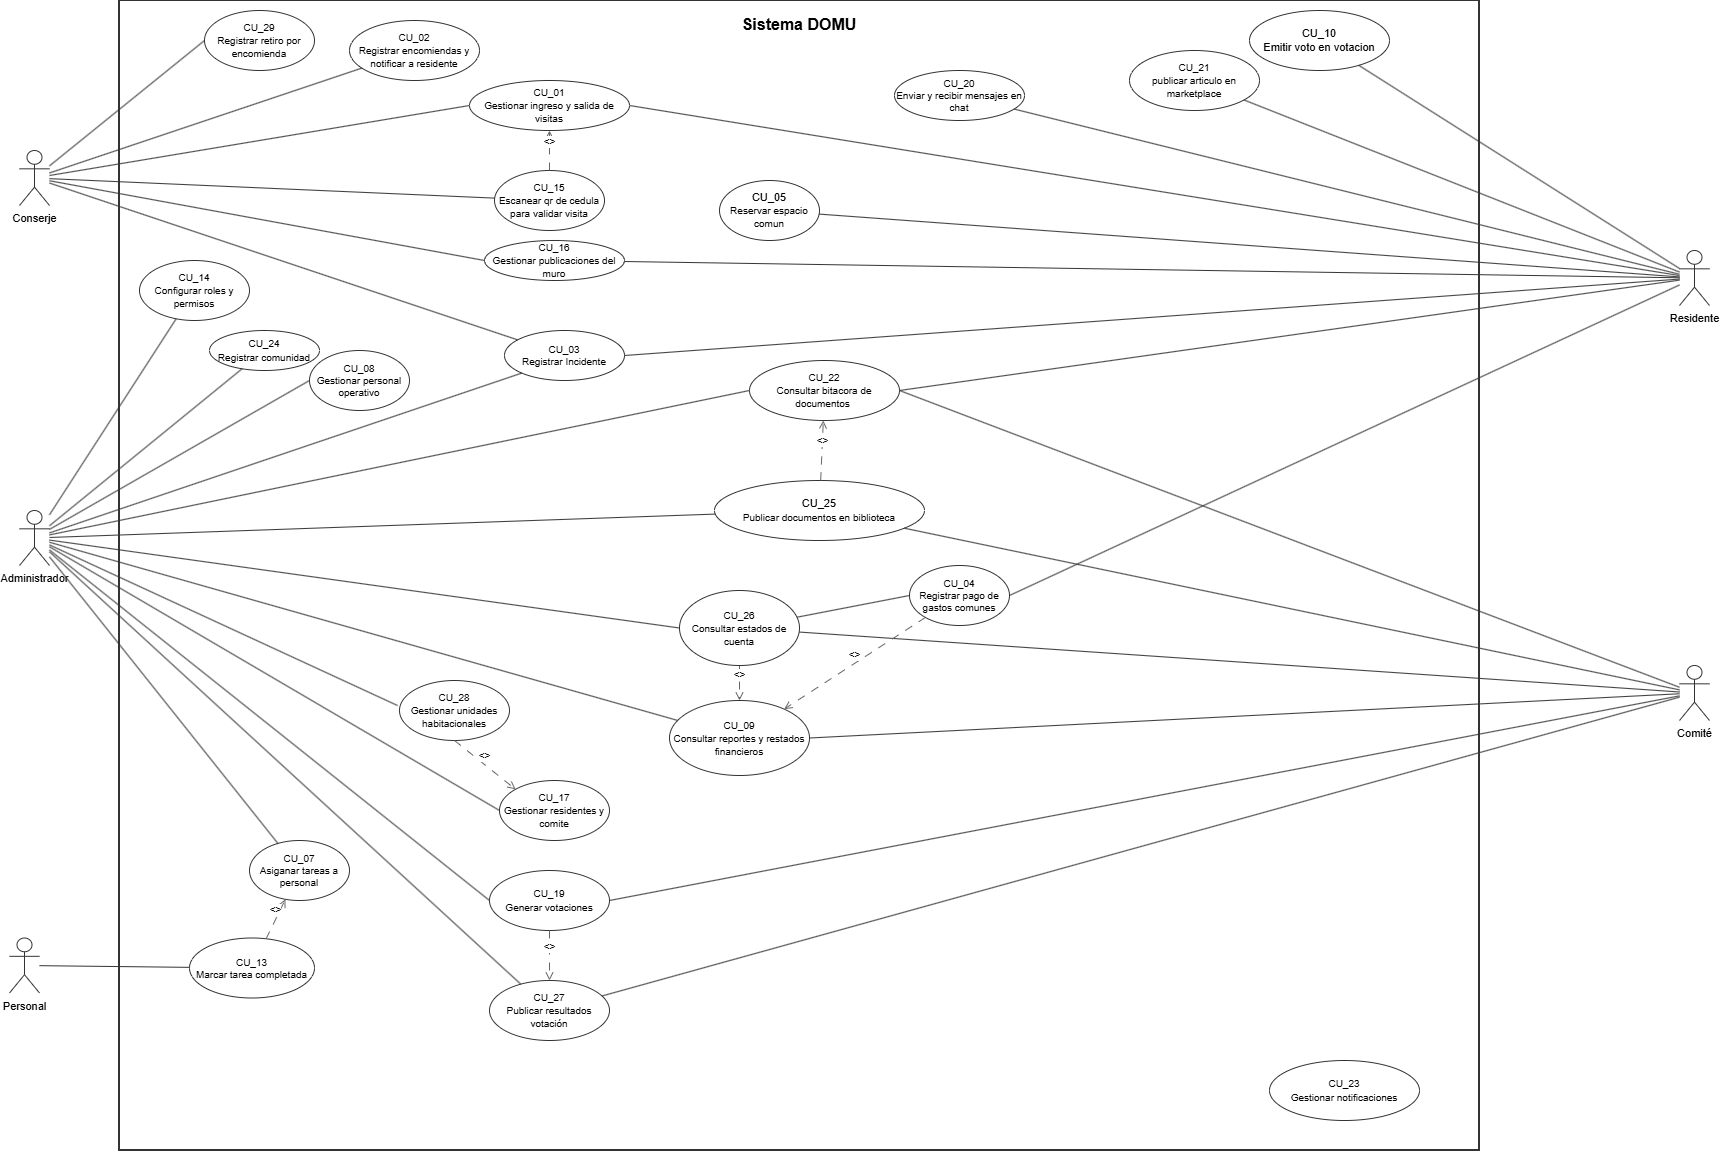
\includegraphics[width=0.98\textwidth]{images/ActoresCU-Diagrama General de Casos de Uso.drawio.png}
  \caption{Diagrama general de los principales casos de uso vigentes del sistema DOMU.}
  \label{fig:diagrama-cu}
\end{figure}

\subsection{Especificacion detallada de Casos de Uso}

% CU_01
\begin{table}[H]\centering
\begin{tabular}{|p{0.475\linewidth}|p{0.475\linewidth}|}\hline
\cutop{CU\_01}{Gestionar ingreso y salida de visitas}
\cusec{Precondiciones}{Residente y/o conserje autenticado segun el punto del flujo; existe una unidad de destino en la comunidad.}
\cusec{Includes}{---}
\cusec{Extends}{CU\_15 Escanear QR de cedula para validar visita, cuando el ingreso se apoya en la lectura del documento de identidad.}
\cuheader{Residente / Conserje}{Sistema}
1) El residente pre-autoriza la visita o el conserje inicia un registro manual al momento del arribo. & 2) Muestra los datos de la visita autorizada o despliega el formulario de registro. \\\hline
3) El conserje identifica a la visita y selecciona la unidad de destino. & 4) Valida datos del visitante, unidad asociada y vigencia del acceso. \\\hline
5) El conserje registra el ingreso o la salida. & 6) Guarda el movimiento y notifica al residente cuando corresponde. \\\hline
\multicolumn{2}{|l|}{\textbf{Flujo de eventos alternativos}}\\\hline
4a. La identificacion es invalida o la unidad no existe. & 4b. Rechaza el registro y solicita corregir los datos. \\\hline
4c. No existe autorizacion previa. & 4d. Permite continuar con registro manual segun validacion de conserjeria. \\\hline
\cusec{Post condiciones}{La visita queda registrada en el sistema con trazabilidad de ingreso y/o salida.}
\end{tabular}
\caption{CU\_01 --- Gestionar ingreso y salida de visitas}
\label{tab:cu01}
\end{table}

% CU_02
\begin{table}[H]\centering
\begin{tabular}{|p{0.475\linewidth}|p{0.475\linewidth}|}\hline
\cutop{CU\_02}{Registrar encomiendas y notificar a residentes}
\cusec{Precondiciones}{Conserje autenticado; la encomienda fue recibida en conserjeria y existe una unidad de destino.}
\cusec{Includes}{---}
\cusec{Extends}{---}
\cuheader{Conserje}{Sistema}
1) Accede al modulo de encomiendas y selecciona registrar recepcion. & 2) Muestra formulario de nueva encomienda. \\\hline
3) Ingresa remitente, descripcion, unidad y evidencia opcional. & 4) Valida los datos y crea la encomienda asociada a la unidad. \\\hline
5) Confirma el registro. & 6) Guarda la encomienda con estado ``Por retirar'' y notifica al residente. \\\hline
\multicolumn{2}{|l|}{\textbf{Flujo de eventos alternativos}}\\\hline
3a. La unidad indicada no existe. & 3b. Muestra error y solicita seleccionar una unidad valida. \\\hline
3c. La evidencia adjunta no es valida. & 3d. Permite continuar sin archivo o solicitar una nueva carga. \\\hline
\cusec{Post condiciones}{La encomienda queda registrada y disponible para seguimiento por conserjeria, administracion y residente.}
\end{tabular}
\caption{CU\_02 --- Registrar encomiendas y notificar a residentes}
\label{tab:cu02}
\end{table}

% CU_03
\begin{table}[H]\centering
\begin{tabular}{|p{0.475\linewidth}|p{0.475\linewidth}|}\hline
\cutop{CU\_03}{Registrar incidente}
\cusec{Precondiciones}{Residente, conserje o administrador autenticado; modulo de incidentes habilitado.}
\cusec{Includes}{---}
\cusec{Extends}{---}
\cuheader{Residente / Conserje / Administrador}{Sistema}
1) Accede al modulo de incidentes. & 2) Muestra el formulario de registro. \\\hline
3) Ingresa categoria, descripcion y antecedentes del incidente. & 4) Valida la informacion minima y permite adjuntar evidencia opcional. \\\hline
5) Confirma el reporte. & 6) Registra el incidente y lo deja disponible para seguimiento por administracion. \\\hline
\multicolumn{2}{|l|}{\textbf{Flujo de eventos alternativos}}\\\hline
3a. Falta informacion obligatoria. & 3b. Indica los campos faltantes y no permite registrar. \\\hline
4a. La evidencia adjunta no cumple formato o tamano. & 4b. Rechaza el archivo y mantiene el formulario para correccion. \\\hline
\cusec{Post condiciones}{Incidente registrado correctamente en el sistema.}
\end{tabular}
\caption{CU\_03 --- Registrar incidente}
\label{tab:cu03}
\end{table}

% CU_04
\begin{table}[H]\centering
\begin{tabular}{|p{0.475\linewidth}|p{0.475\linewidth}|}\hline
\cutop{CU\_04}{Registrar pago de gastos comunes}
\cusec{Precondiciones}{Residente autenticado; existe al menos un periodo pendiente de pago.}
\cusec{Includes}{CU\_09 Consultar reportes y estados financieros.}
\cusec{Extends}{---}
\cuheader{Residente / Administrador}{Sistema}
1) El residente selecciona el periodo pendiente que desea pagar. & 2) Muestra el detalle del estado de cuenta, cargos y saldo pendiente. \\\hline
3) El residente adjunta el comprobante de transferencia y confirma el envio. & 4) Valida el archivo y registra el pago con estado ``Pendiente de validacion''. \\\hline
5) El administrador revisa el comprobante asociado al periodo. & 6) Aprueba manualmente el pago y cambia el estado a ``Pagado'', o lo observa para una nueva carga. \\\hline
\multicolumn{2}{|l|}{\textbf{Flujo de eventos alternativos}}\\\hline
3a. El archivo no cumple con el formato esperado. & 3b. Rechaza la carga y solicita un nuevo comprobante. \\\hline
5a. El comprobante no es valido o no coincide con el cargo. & 5b. Mantiene el estado pendiente de validacion y registra observacion administrativa. \\\hline
\cusec{Post condiciones}{El comprobante queda asociado al periodo y el pago queda pendiente o validado segun la revision administrativa.}
\end{tabular}
\caption{CU\_04 --- Registrar pago de gastos comunes}
\label{tab:cu04}
\end{table}

% CU_05
\begin{table}[H]\centering
\begin{tabular}{|p{0.475\linewidth}|p{0.475\linewidth}|}\hline
\cutop{CU\_05}{Reservar espacio comun}
\cusec{Precondiciones}{Residente autenticado; existen espacios comunes y franjas horarias configuradas.}
\cusec{Includes}{---}
\cusec{Extends}{---}
\cuheader{Residente}{Sistema}
1) Selecciona el espacio comun y la fecha deseada. & 2) Muestra disponibilidad por bloque horario. \\\hline
3) Elige un horario y confirma la reserva. & 4) Valida reglas de disponibilidad, aforo y restricciones por mora. \\\hline
5) Finaliza la solicitud. & 6) Registra la reserva y actualiza el calendario del espacio comun. \\\hline
\multicolumn{2}{|l|}{\textbf{Flujo de eventos alternativos}}\\\hline
4a. El horario ya no esta disponible. & 4b. Informa el conflicto y ofrece horarios alternativos. \\\hline
4c. El residente tiene bloqueo por mora. & 4d. Deniega la reserva e informa el motivo. \\\hline
\cusec{Post condiciones}{El espacio queda reservado para la fecha y bloque seleccionado.}
\end{tabular}
\caption{CU\_05 --- Reservar espacio comun}
\label{tab:cu05}
\end{table}

% CU_07
\begin{table}[H]\centering
\begin{tabular}{|p{0.475\linewidth}|p{0.475\linewidth}|}\hline
\cutop{CU\_07}{Asignar tareas a personal}
\cusec{Precondiciones}{Administrador autenticado; existe personal operativo activo en el sistema.}
\cusec{Includes}{---}
\cusec{Extends}{CU\_13 Marcar tarea completada.}
\cuheader{Administrador}{Sistema}
1) Ingresa al modulo de tareas y crea una nueva tarea. & 2) Muestra formulario de definicion y asignacion. \\\hline
3) Ingresa descripcion, prioridad, fecha limite y responsable. & 4) Valida la informacion y registra la tarea. \\\hline
5) Confirma la asignacion. & 6) Notifica al personal responsable y deja la tarea en estado ``Asignada''. \\\hline
\multicolumn{2}{|l|}{\textbf{Flujo de eventos alternativos}}\\\hline
3a. Falta descripcion o responsable. & 3b. Solicita completar los campos obligatorios. \\\hline
\cusec{Post condiciones}{La tarea queda asignada y visible para el personal operativo correspondiente.}
\end{tabular}
\caption{CU\_07 --- Asignar tareas a personal}
\label{tab:cu07}
\end{table}

% CU_08
\begin{table}[H]\centering
\begin{tabular}{|p{0.475\linewidth}|p{0.475\linewidth}|}\hline
\cutop{CU\_08}{Gestionar personal operativo}
\cusec{Precondiciones}{Administrador autenticado; comunidad activa.}
\cusec{Includes}{---}
\cusec{Extends}{---}
\cuheader{Administrador}{Sistema}
1) Accede al modulo de personal operativo. & 2) Muestra listado del personal registrado y acciones disponibles. \\\hline
3) Crea, edita o elimina un registro de personal. & 4) Valida la informacion y actualiza el registro correspondiente. \\\hline
5) Asigna el rol o tipo de personal (conserje, aseo, mantencion u otro). & 6) Guarda los cambios y actualiza la disponibilidad del personal en el sistema. \\\hline
\multicolumn{2}{|l|}{\textbf{Flujo de eventos alternativos}}\\\hline
3a. El correo o identificador ya existe. & 3b. Informa el conflicto y solicita correccion. \\\hline
3c. Se intenta eliminar personal con dependencias activas. & 3d. Solicita resolver las dependencias antes de completar la operacion. \\\hline
\cusec{Post condiciones}{El personal operativo queda actualizado segun las acciones realizadas por administracion.}
\end{tabular}
\caption{CU\_08 --- Gestionar personal operativo}
\label{tab:cu08}
\end{table}

% CU_09
\begin{table}[H]\centering
\begin{tabular}{|p{0.475\linewidth}|p{0.475\linewidth}|}\hline
\cutop{CU\_09}{Consultar reportes y estados financieros}
\cusec{Precondiciones}{Administrador o Comite autenticado; existen periodos y cargos registrados en el sistema.}
\cusec{Includes}{---}
\cusec{Extends}{---}
\cuheader{Administrador / Comite}{Sistema}
1) Ingresa al modulo financiero o panel de reportes. & 2) Lista periodos, estados de cuenta, pagos y documentos disponibles. \\\hline
3) Selecciona el periodo, unidad o vista financiera a revisar. & 4) Muestra cargos, pagos, saldo, resumen del periodo y estadisticas disponibles. \\\hline
5) Solicita descargar o visualizar el documento asociado. & 6) Genera o entrega el archivo disponible y registra la consulta para trazabilidad. \\\hline
\multicolumn{2}{|l|}{\textbf{Flujo de eventos alternativos}}\\\hline
2a. No existen periodos publicados para el filtro seleccionado. & 2b. Informa que no hay informacion disponible para el rango solicitado. \\\hline
5a. El documento no esta generado. & 5b. Muestra el detalle en pantalla y registra la falta del archivo exportable. \\\hline
\cusec{Post condiciones}{La informacion financiera queda consultada y, cuando existe soporte documental, puede descargarse desde el sistema.}
\end{tabular}
\caption{CU\_09 --- Consultar reportes y estados financieros}
\label{tab:cu09}
\end{table}

% CU_10
\begin{table}[H]\centering
\begin{tabular}{|p{0.475\linewidth}|p{0.475\linewidth}|}\hline
\cutop{CU\_10}{Emitir voto en votacion comunitaria}
\cusec{Precondiciones}{Residente autenticado; existe una votacion abierta y habilitada para su participacion.}
\cusec{Includes}{---}
\cusec{Extends}{---}
\cuheader{Residente}{Sistema}
1) Ingresa al modulo de votaciones. & 2) Lista las votaciones abiertas y sus antecedentes. \\\hline
3) Selecciona una votacion y revisa las opciones disponibles. & 4) Valida habilitacion, registra el voto y actualiza el estado de participacion. \\\hline
5) Confirma su opcion. & 6) Guarda el voto y deja trazabilidad del sufragio emitido. \\\hline
\multicolumn{2}{|l|}{\textbf{Flujo de eventos alternativos}}\\\hline
4a. El residente ya voto. & 4b. Informa que la votacion ya fue respondida y bloquea un nuevo envio. \\\hline
4c. La votacion se encuentra cerrada. & 4d. Muestra solo los resultados o el estado historico, sin permitir votar. \\\hline
\cusec{Post condiciones}{El voto queda registrado correctamente para la votacion seleccionada.}
\end{tabular}
\caption{CU\_10 --- Emitir voto en votacion comunitaria}
\label{tab:cu10}
\end{table}

% CU_13
\begin{table}[H]\centering
\begin{tabular}{|p{0.475\linewidth}|p{0.475\linewidth}|}\hline
\cutop{CU\_13}{Marcar tarea completada}
\cusec{Precondiciones}{Personal operativo autenticado; existe una tarea asignada en estado pendiente o en progreso.}
\cusec{Includes}{---}
\cusec{Extends}{---}
\cuheader{Personal operativo}{Sistema}
1) Accede a la tarea asignada. & 2) Muestra detalle, prioridad y fecha comprometida. \\\hline
3) Marca la tarea como completada y adjunta evidencia si corresponde. & 4) Actualiza el estado de la tarea y registra fecha de cierre. \\\hline
5) Confirma el cierre. & 6) Notifica a administracion que la tarea fue completada. \\\hline
\multicolumn{2}{|l|}{\textbf{Flujo de eventos alternativos}}\\\hline
3a. La evidencia no cumple con el formato permitido. & 3b. Solicita una nueva carga o permite cerrar sin adjunto. \\\hline
\cusec{Post condiciones}{La tarea queda cerrada o avanzada con respaldo operacional en el sistema.}
\end{tabular}
\caption{CU\_13 --- Marcar tarea completada}
\label{tab:cu13}
\end{table}

% CU_14
\begin{table}[H]\centering
\begin{tabular}{|p{0.475\linewidth}|p{0.475\linewidth}|}\hline
\cutop{CU\_14}{Configurar roles y permisos}
\cusec{Precondiciones}{Administrador autenticado con privilegios de seguridad.}
\cusec{Includes}{---}
\cusec{Extends}{---}
\cuheader{Administrador}{Sistema}
1) Accede a la configuracion de roles y permisos. & 2) Muestra roles disponibles y permisos asociados por modulo. \\\hline
3) Crea o ajusta permisos de un rol existente. & 4) Valida consistencia de la configuracion y guarda la politica de acceso. \\\hline
5) Asigna el rol correspondiente a un usuario. & 6) Actualiza permisos efectivos y deja registro de auditoria. \\\hline
\multicolumn{2}{|l|}{\textbf{Flujo de eventos alternativos}}\\\hline
3a. La configuracion genera conflicto de permisos. & 3b. Informa la colision y no aplica los cambios hasta su correccion. \\\hline
\cusec{Post condiciones}{La configuracion de acceso queda actualizada y trazada.}
\end{tabular}
\caption{CU\_14 --- Configurar roles y permisos}
\label{tab:cu14}
\end{table}

% CU_15
\begin{table}[H]\centering
\begin{tabular}{|p{0.475\linewidth}|p{0.475\linewidth}|}\hline
\cutop{CU\_15}{Escanear QR de cedula para validar visita}
\cusec{Precondiciones}{Conserje autenticado; la visita presenta una cedula de identidad chilena con QR legible; el lector QR se encuentra operativo.}
\cusec{Includes}{---}
\cusec{Extends}{CU\_01 Gestionar ingreso y salida de visitas.}
\cuheader{Conserje}{Sistema}
1) Escanea el QR de la cedula del visitante. & 2) Extrae RUN y datos de identificacion disponibles desde el documento. \\\hline
3) Solicita la validacion del documento. & 4) Busca coincidencias con registros previos y autocompleta el formulario de visita. \\\hline
5) Confirma el uso de los datos recuperados. & 6) Deja la identificacion lista para continuar el flujo de ingreso. \\\hline
\multicolumn{2}{|l|}{\textbf{Flujo de eventos alternativos}}\\\hline
2a. El QR no puede leerse o esta incompleto. & 2b. Informa el error y permite continuar con ingreso manual de datos. \\\hline
\cusec{Post condiciones}{La identidad del visitante queda validada o precargada para el registro de la visita.}
\end{tabular}
\caption{CU\_15 --- Escanear QR de cedula para validar visita}
\label{tab:cu15}
\end{table}

% CU_16
\begin{table}[H]\centering
\begin{tabular}{|p{0.475\linewidth}|p{0.475\linewidth}|}\hline
\cutop{CU\_16}{Gestionar publicaciones del muro comunitario}
\cusec{Precondiciones}{Administrador o residente autenticado; modulo de publicaciones habilitado.}
\cusec{Includes}{---}
\cusec{Extends}{---}
\cuheader{Administrador / Residente}{Sistema}
1) El administrador accede al muro para publicar, o el residente ingresa para revisar publicaciones vigentes. & 2) Muestra el listado del muro y, para administracion, el formulario de nueva publicacion. \\\hline
3) El administrador ingresa categoria, titulo y contenido del aviso. & 4) Valida los datos y publica el contenido en el muro de la comunidad. \\\hline
5) El residente consulta, filtra o abre una publicacion. & 6) Despliega el contenido y registra la visualizacion en el contexto de la comunidad. \\\hline
\multicolumn{2}{|l|}{\textbf{Flujo de eventos alternativos}}\\\hline
3a. Faltan campos obligatorios de la publicacion. & 3b. Informa el error y mantiene el formulario para correccion. \\\hline
5a. No existen publicaciones vigentes. & 5b. Muestra estado vacio del muro comunitario. \\\hline
\cusec{Post condiciones}{Las publicaciones quedan visibles para los residentes y disponibles para consulta posterior.}
\end{tabular}
\caption{CU\_16 --- Gestionar publicaciones del muro comunitario}
\label{tab:cu16}
\end{table}

% CU_17
\begin{table}[H]\centering
\begin{tabular}{|p{0.475\linewidth}|p{0.475\linewidth}|}\hline
\cutop{CU\_17}{Gestionar residentes y comite}
\cusec{Precondiciones}{Administrador autenticado; comunidad activa y modulos administrativos disponibles.}
\cusec{Includes}{CU\_28 Gestionar unidades habitacionales, cuando se requiere asignar o reasignar una unidad.}
\cusec{Extends}{---}
\cuheader{Administrador}{Sistema}
1) Accede al modulo de usuarios de la comunidad. & 2) Muestra listado de residentes y miembros del comite registrados. \\\hline
3) Crea o edita la ficha del usuario comunitario. & 4) Valida datos personales, rol y estado del registro. \\\hline
5) Asigna rol de residente o comite y vincula la unidad cuando corresponde. & 6) Guarda los cambios y actualiza la informacion visible para la comunidad. \\\hline
\multicolumn{2}{|l|}{\textbf{Flujo de eventos alternativos}}\\\hline
3a. El correo o documento ya existe en la comunidad. & 3b. Informa el conflicto y no permite duplicar el registro. \\\hline
5a. La unidad seleccionada no esta disponible. & 5b. Solicita escoger otra unidad o revisar la asociacion actual. \\\hline
\cusec{Post condiciones}{La informacion de residentes y comite queda actualizada y vinculada a la comunidad activa.}
\end{tabular}
\caption{CU\_17 --- Gestionar residentes y comite}
\label{tab:cu17}
\end{table}

% CU_19
\begin{table}[H]\centering
\begin{tabular}{|p{0.475\linewidth}|p{0.475\linewidth}|}\hline
\cutop{CU\_19}{Gestionar votaciones comunitarias}
\cusec{Precondiciones}{Administrador o Comite autenticado; modulo de votaciones habilitado.}
\cusec{Includes}{---}
\cusec{Extends}{CU\_27 Publicar resultados de votacion, una vez cerrada la votacion.}
\cuheader{Administrador / Comite}{Sistema}
1) Ingresa al modulo de votaciones y selecciona crear o administrar una votacion. & 2) Muestra historial, estado actual y formulario de configuracion. \\\hline
3) Define titulo, descripcion, opciones y fecha de cierre. & 4) Valida el formulario y registra la votacion en estado abierta. \\\hline
5) Publica o cierra la votacion segun corresponda. & 6) Notifica a la comunidad y actualiza el historial del proceso. \\\hline
\multicolumn{2}{|l|}{\textbf{Flujo de eventos alternativos}}\\\hline
3a. Hay menos de dos opciones o la fecha no es valida. & 3b. Solicita corregir la configuracion antes de publicar. \\\hline
\cusec{Post condiciones}{La votacion queda creada, administrada o cerrada segun la accion ejecutada.}
\end{tabular}
\caption{CU\_19 --- Gestionar votaciones comunitarias}
\label{tab:cu19}
\end{table}

% CU_20
\begin{table}[H]\centering
\begin{tabular}{|p{0.475\linewidth}|p{0.475\linewidth}|}\hline
\cutop{CU\_20}{Enviar y recibir mensajes en chat}
\cusec{Precondiciones}{Residente autenticado; canal de chat habilitado en la comunidad.}
\cusec{Includes}{---}
\cusec{Extends}{---}
\cuheader{Residente}{Sistema}
1) Accede al modulo de chat y selecciona una conversacion o inicia una nueva. & 2) Muestra salas disponibles y el historial del chat seleccionado. \\\hline
3) Escribe y envia un mensaje. & 4) Transmite el mensaje en tiempo real y lo almacena en el historial. \\\hline
5) Recibe nuevas respuestas. & 6) Actualiza el estado de lectura y notifica actividad cuando corresponde. \\\hline
\multicolumn{2}{|l|}{\textbf{Flujo de eventos alternativos}}\\\hline
3a. La conversacion no esta disponible o fue ocultada. & 3b. Informa el estado y bloquea el envio hasta recuperar acceso. \\\hline
\cusec{Post condiciones}{La conversacion queda actualizada con los mensajes intercambiados.}
\end{tabular}
\caption{CU\_20 --- Enviar y recibir mensajes en chat}
\label{tab:cu20}
\end{table}

% CU_21
\begin{table}[H]\centering
\begin{tabular}{|p{0.475\linewidth}|p{0.475\linewidth}|}\hline
\cutop{CU\_21}{Publicar articulo en marketplace}
\cusec{Precondiciones}{Residente autenticado; marketplace comunitario habilitado.}
\cusec{Includes}{---}
\cusec{Extends}{---}
\cuheader{Residente}{Sistema}
1) Accede al marketplace y selecciona crear publicacion. & 2) Muestra formulario de articulo y carga de imagenes. \\\hline
3) Ingresa titulo, descripcion, precio y fotos. & 4) Valida la informacion y almacena la publicacion. \\\hline
5) Publica, edita o elimina el articulo. & 6) Actualiza el listado comunitario y deja trazabilidad del anuncio. \\\hline
\multicolumn{2}{|l|}{\textbf{Flujo de eventos alternativos}}\\\hline
3a. Las imagenes no cumplen el formato permitido. & 3b. Rechaza los archivos y solicita una nueva carga. \\\hline
\cusec{Post condiciones}{El articulo queda disponible en el marketplace o actualizado segun la accion realizada.}
\end{tabular}
\caption{CU\_21 --- Publicar articulo en marketplace}
\label{tab:cu21}
\end{table}

% CU_22
\begin{table}[H]\centering
\begin{tabular}{|p{0.475\linewidth}|p{0.475\linewidth}|}\hline
\cutop{CU\_22}{Consultar biblioteca de documentos}
\cusec{Precondiciones}{Administrador, residente o Comite autenticado; existen documentos publicados en la biblioteca.}
\cusec{Includes}{---}
\cusec{Extends}{---}
\cuheader{Administrador / Residente / Comite}{Sistema}
1) Accede al modulo Biblioteca. & 2) Lista documentos disponibles por categoria y nombre. \\\hline
3) Filtra o selecciona un documento. & 4) Permite visualizarlo o descargarlo desde el repositorio documental. \\\hline
\multicolumn{2}{|l|}{\textbf{Flujo de eventos alternativos}}\\\hline
4a. El archivo no se encuentra disponible. & 4b. Informa el problema y mantiene el documento como no descargable. \\\hline
\cusec{Post condiciones}{El documento queda consultado o descargado por el actor correspondiente.}
\end{tabular}
\caption{CU\_22 --- Consultar biblioteca de documentos}
\label{tab:cu22}
\end{table}

% CU_23
\begin{table}[H]\centering
\begin{tabular}{|p{0.475\linewidth}|p{0.475\linewidth}|}\hline
\cutop{CU\_23}{Gestionar notificaciones}
\cusec{Precondiciones}{Usuario autenticado.}
\cusec{Includes}{---}
\cusec{Extends}{---}
\cuheader{Usuario}{Sistema}
1) Abre el centro de notificaciones. & 2) Muestra notificaciones ordenadas por fecha y tipo. \\\hline
3) Marca notificaciones como leidas o ajusta preferencias. & 4) Actualiza el estado de lectura y la configuracion asociada. \\\hline
\multicolumn{2}{|l|}{\textbf{Flujo de eventos alternativos}}\\\hline
2a. No existen notificaciones para el usuario. & 2b. Muestra estado vacio y mantiene accesibles las preferencias. \\\hline
\cusec{Post condiciones}{El estado de lectura y las preferencias de notificacion quedan actualizados.}
\end{tabular}
\caption{CU\_23 --- Gestionar notificaciones}
\label{tab:cu23}
\end{table}

% CU_24
\begin{table}[H]\centering
\begin{tabular}{|p{0.475\linewidth}|p{0.475\linewidth}|}\hline
\cutop{CU\_24}{Registrar y aprobar comunidad}
\cusec{Precondiciones}{Solicitante con informacion de la comunidad y documentacion de respaldo.}
\cusec{Includes}{---}
\cusec{Extends}{---}
\cuheader{Administrador}{Sistema}
1) Completa el formulario de solicitud de comunidad. & 2) Valida los datos y almacena los documentos adjuntos. \\\hline
3) Envia la solicitud. & 4) Notifica al flujo de aprobacion mediante correo electronico. \\\hline
5) El aprobador revisa y aprueba o rechaza la solicitud. & 6) Crea la comunidad y habilita la invitacion para el administrador responsable. \\\hline
\multicolumn{2}{|l|}{\textbf{Flujo de eventos alternativos}}\\\hline
5a. La solicitud es rechazada. & 5b. Registra el motivo e informa el resultado al solicitante. \\\hline
\cusec{Post condiciones}{La comunidad queda creada o rechazada con trazabilidad del proceso de aprobacion.}
\end{tabular}
\caption{CU\_24 --- Registrar y aprobar comunidad}
\label{tab:cu24}
\end{table}

% CU_25
\begin{table}[H]\centering
\begin{tabular}{|p{0.475\linewidth}|p{0.475\linewidth}|}\hline
\cutop{CU\_25}{Publicar documentos y actas en la biblioteca}
\cusec{Precondiciones}{Administrador o Comite autenticado; modulo Biblioteca habilitado.}
\cusec{Includes}{CU\_22 Consultar biblioteca de documentos.}
\cusec{Extends}{---}
\cuheader{Administrador / Comite}{Sistema}
1) Accede a la biblioteca y selecciona cargar documento. & 2) Muestra formulario de nombre, categoria y archivo. \\\hline
3) Adjunta el documento y define su categoria. & 4) Valida formato, metadatos y permisos de carga. \\\hline
5) Confirma la publicacion. & 6) Guarda el documento y lo deja disponible para consulta en la comunidad. \\\hline
\multicolumn{2}{|l|}{\textbf{Flujo de eventos alternativos}}\\\hline
4a. El archivo no es valido o supera el limite permitido. & 4b. Rechaza la carga y solicita un nuevo archivo. \\\hline
4c. El Comite intenta usar una categoria distinta de ``actas''. & 4d. Restringe la categoria y solicita ajustarla a ``actas''. \\\hline
\cusec{Post condiciones}{El documento queda publicado en la biblioteca documental de la comunidad.}
\end{tabular}
\caption{CU\_25 --- Publicar documentos y actas en la biblioteca}
\label{tab:cu25}
\end{table}

% CU_26
\begin{table}[H]\centering
\begin{tabular}{|p{0.475\linewidth}|p{0.475\linewidth}|}\hline
\cutop{CU\_26}{Consultar estados de cuenta para fiscalizacion}
\cusec{Precondiciones}{Comite o administrador autenticado; existen periodos financieros publicados para consulta.}
\cusec{Includes}{CU\_09 Consultar reportes y estados financieros.}
\cusec{Extends}{---}
\cuheader{Comite / Administrador}{Sistema}
1) Ingresa al modulo financiero en modo consulta. & 2) Lista periodos y estados de cuenta disponibles. \\\hline
3) Selecciona el periodo que desea fiscalizar. & 4) Muestra detalle de cargos, pagos, saldo y documentos asociados. \\\hline
5) Consulta o descarga el respaldo disponible. & 6) Registra la accion para fines de trazabilidad y fiscalizacion. \\\hline
\multicolumn{2}{|l|}{\textbf{Flujo de eventos alternativos}}\\\hline
2a. El periodo aun no fue publicado. & 2b. Informa indisponibilidad del estado de cuenta solicitado. \\\hline
\cusec{Post condiciones}{El estado de cuenta queda consultado sin modificar la informacion financiera del sistema.}
\end{tabular}
\caption{CU\_26 --- Consultar estados de cuenta para fiscalizacion}
\label{tab:cu26}
\end{table}

% CU_27
\begin{table}[H]\centering
\begin{tabular}{|p{0.475\linewidth}|p{0.475\linewidth}|}\hline
\cutop{CU\_27}{Publicar resultados de votacion}
\cusec{Precondiciones}{Administrador o Comite autenticado; existe una votacion cerrada con resultados consolidados.}
\cusec{Includes}{---}
\cusec{Extends}{CU\_19 Gestionar votaciones comunitarias.}
\cuheader{Administrador / Comite}{Sistema}
1) Selecciona una votacion cerrada. & 2) Muestra resultados consolidados, total de votos y estado del proceso. \\\hline
3) Confirma la publicacion de resultados. & 4) Deja disponible el resultado en el historial y permite su descarga o consulta. \\\hline
5) Comunica el cierre a la comunidad. & 6) Registra la publicacion y notifica el resultado cuando corresponde. \\\hline
\multicolumn{2}{|l|}{\textbf{Flujo de eventos alternativos}}\\\hline
2a. La votacion aun esta abierta. & 2b. Impide la publicacion y exige cerrar primero el proceso. \\\hline
\cusec{Post condiciones}{Los resultados quedan publicados y disponibles para consulta historica.}
\end{tabular}
\caption{CU\_27 --- Publicar resultados de votacion}
\label{tab:cu27}
\end{table}

% CU_28
\begin{table}[H]\centering
\begin{tabular}{|p{0.475\linewidth}|p{0.475\linewidth}|}\hline
\cutop{CU\_28}{Gestionar unidades habitacionales}
\cusec{Precondiciones}{Administrador autenticado; comunidad activa.}
\cusec{Includes}{---}
\cusec{Extends}{---}
\cuheader{Administrador}{Sistema}
1) Accede al modulo de unidades habitacionales. & 2) Muestra listado de unidades y opciones de creacion o edicion. \\\hline
3) Crea, edita o elimina una unidad. & 4) Valida numero, torre, piso y metadatos asociados a la unidad. \\\hline
5) Asocia o desvincula residentes cuando corresponde. & 6) Guarda los cambios y actualiza la estructura habitacional de la comunidad. \\\hline
\multicolumn{2}{|l|}{\textbf{Flujo de eventos alternativos}}\\\hline
3a. Se intenta eliminar una unidad con residentes asociados. & 3b. Impide la eliminacion y solicita desvincular primero a los residentes. \\\hline
\cusec{Post condiciones}{Las unidades habitacionales quedan actualizadas y disponibles para operacion administrativa.}
\end{tabular}
\caption{CU\_28 --- Gestionar unidades habitacionales}
\label{tab:cu28}
\end{table}

% CU_29
\begin{table}[H]\centering
\begin{tabular}{|p{0.475\linewidth}|p{0.475\linewidth}|}\hline
\cutop{CU\_29}{Registrar retiro de encomienda}
\cusec{Precondiciones}{Conserje autenticado; existe una encomienda en estado ``Por retirar''.}
\cusec{Includes}{---}
\cusec{Extends}{---}
\cuheader{Conserje}{Sistema}
1) Busca la encomienda pendiente de retiro. & 2) Muestra el detalle de la encomienda y la unidad asociada. \\\hline
3) Verifica al residente o persona autorizada. & 4) Valida que la encomienda siga disponible para entrega. \\\hline
5) Marca la encomienda como retirada. & 6) Registra fecha y hora del retiro y actualiza el estado a ``Retirada''. \\\hline
\multicolumn{2}{|l|}{\textbf{Flujo de eventos alternativos}}\\\hline
4a. La encomienda ya fue retirada. & 4b. Informa el estado actual y bloquea un nuevo cierre. \\\hline
4c. No es posible validar al receptor. & 4d. Mantiene la encomienda en estado ``Por retirar''. \\\hline
\cusec{Post condiciones}{La encomienda queda entregada y con trazabilidad del retiro en el sistema.}
\end{tabular}
\caption{CU\_29 --- Registrar retiro de encomienda}
\label{tab:cu29}
\end{table}

% \subsection{Diagramas de casos de uso por modulo}

% A continuacion se presentan diagramas resumidos por modulo funcional. Se mantienen como apoyo visual del analisis vigente y excluyen los casos de uso diferidos al Anexo~\ref{anexo:casos-restantes}.

% \begin{figure}[H]
%   \centering
%   \fbox{\parbox{0.85\textwidth}{\centering\vspace{3.2cm}
%   \textit{Modulo Visitas y Acceso: CU\_01 y CU\_15.}\\
%   \textit{Actores principales: Residente y Conserje.}
%   \vspace{3.2cm}}}
%   \caption{Diagrama de casos de uso --- Modulo Visitas y Acceso.}
%   \label{fig:cu-modulo-visitas}
% \end{figure}

% \begin{figure}[H]
%   \centering
%   \fbox{\parbox{0.85\textwidth}{\centering\vspace{3.2cm}
%   \textit{Modulo Encomiendas e Incidentes: CU\_02, CU\_03 y CU\_29.}\\
%   \textit{Actores principales: Conserje, Residente y Administrador.}
%   \vspace{3.2cm}}}
%   \caption{Diagrama de casos de uso --- Modulo Encomiendas e Incidentes.}
%   \label{fig:cu-modulo-encomiendas}
% \end{figure}

% \begin{figure}[H]
%   \centering
%   \fbox{\parbox{0.85\textwidth}{\centering\vspace{3.2cm}
%   \textit{Modulo Financiero: CU\_04, CU\_09 y CU\_26.}\\
%   \textit{Actores principales: Residente, Administrador y Comite.}
%   \vspace{3.2cm}}}
%   \caption{Diagrama de casos de uso --- Modulo Financiero.}
%   \label{fig:cu-modulo-financiero}
% \end{figure}

% \begin{figure}[H]
%   \centering
%   \fbox{\parbox{0.85\textwidth}{\centering\vspace{3.2cm}
%   \textit{Modulo Comunidad: CU\_10, CU\_16, CU\_19, CU\_20, CU\_21, CU\_22, CU\_25 y CU\_27.}\\
%   \textit{Actores principales: Residente, Administrador y Comite.}
%   \vspace{3.2cm}}}
%   \caption{Diagrama de casos de uso --- Modulo Comunidad y Gobernanza.}
%   \label{fig:cu-modulo-comunidad}
% \end{figure}

% \begin{figure}[H]
%   \centering
%   \fbox{\parbox{0.85\textwidth}{\centering\vspace{3.2cm}
%   \textit{Modulo Administrativo: CU\_07, CU\_08, CU\_14, CU\_17, CU\_24 y CU\_28.}\\
%   \textit{Actores principales: Administrador y Personal operativo.}
%   \vspace{3.2cm}}}
%   \caption{Diagrama de casos de uso --- Modulo Administrativo.}
%   \label{fig:cu-modulo-admin}
% \end{figure}

\section{Matriz de trazabilidad RF--CU}

\begin{longtable}{|m{3cm}|m{12.5cm}|}
\hline
\textbf{RF} & \textbf{Casos de Uso relacionados} \\\hline
RF\_01 (Visitas) & CU\_01, CU\_15 \\\hline
RF\_02 (Notificaciones push) & CU\_01, CU\_02, CU\_03, CU\_04, CU\_07, CU\_13, CU\_19, CU\_23, CU\_29 \\\hline
RF\_03 (Pre-autorizacion de visitas) & CU\_01, CU\_15 \\\hline
RF\_04 (Encomiendas) & CU\_02, CU\_29 \\\hline
RF\_05 (Tareas del personal) & CU\_07, CU\_08, CU\_13 \\\hline
RF\_06 (Inicio/fin jornada) & Cobertura parcial en v1.0 mediante CU\_13; la marcacion de jornada queda diferida al anexo. \\\hline
RF\_07 (Estado de cuenta y pago) & CU\_04, CU\_09, CU\_26 \\\hline
RF\_08 (Morosidad/conciliacion) & Sin CU vigente en el cuerpo principal; vease Anexo~\ref{anexo:casos-restantes} (CU\_06). \\\hline
RF\_09 (Reservas) & CU\_05 \\\hline
RF\_10 (Votaciones) & CU\_10, CU\_19, CU\_27 \\\hline
RF\_11 (Comunicacion comunitaria) & CU\_16, CU\_20 \\\hline
RF\_12 (Tickets de reclamos) & CU\_03 \\\hline
RF\_13 (Gestion de votaciones por Administracion/Comite) & CU\_19, CU\_27 \\\hline
RF\_14 (Mantenimiento preventivo) & Sin CU vigente en el cuerpo principal; vease Anexo~\ref{anexo:casos-restantes} (CU\_11 y CU\_18). \\\hline
RF\_15 (Dashboards/KPI) & CU\_09 \\\hline
RF\_16 (RBAC y configuracion administrativa) & CU\_14, CU\_17, CU\_24, CU\_28 \\\hline
RF\_17 (Chat en tiempo real) & CU\_20 \\\hline
RF\_18 (Marketplace) & CU\_21 \\\hline
RF\_19 (Biblioteca documental) & CU\_22, CU\_25 \\\hline
RF\_20 (Notificaciones en tiempo real) & CU\_01, CU\_02, CU\_03, CU\_04, CU\_07, CU\_13, CU\_19, CU\_23, CU\_29 \\\hline
\caption{Matriz de trazabilidad RF--CU de la version vigente.}
\label{tab:traza-compacta}
\end{longtable}

\begin{landscape}
\scriptsize
\setlength{\tabcolsep}{2pt}
\renewcommand{\arraystretch}{1.1}
\begin{longtable}{|l|*{25}{c|}}
\hline
\textbf{RF \textbackslash\ CU} & \textbf{01} & \textbf{02} & \textbf{03} & \textbf{04} & \textbf{05} & \textbf{07} & \textbf{08} & \textbf{09} & \textbf{10} & \textbf{13} & \textbf{14} & \textbf{15} & \textbf{16} & \textbf{17} & \textbf{19} & \textbf{20} & \textbf{21} & \textbf{22} & \textbf{23} & \textbf{24} & \textbf{25} & \textbf{26} & \textbf{27} & \textbf{28} & \textbf{29}\\\hline
RF\_01 & X &  &  &  &  &  &  &  &  &  &  & X &  &  &  &  &  &  &  &  &  &  &  &  &  \\\hline
RF\_02 & X & X & X & X &  & X &  &  &  & X &  &  &  &  & X &  &  &  & X &  &  &  &  &  & X \\\hline
RF\_03 & X &  &  &  &  &  &  &  &  &  &  & X &  &  &  &  &  &  &  &  &  &  &  &  &  \\\hline
RF\_04 &  & X &  &  &  &  &  &  &  &  &  &  &  &  &  &  &  &  &  &  &  &  &  &  & X \\\hline
RF\_05 &  &  &  &  &  & X & X &  &  & X &  &  &  &  &  &  &  &  &  &  &  &  &  &  &  \\\hline
RF\_06 &  &  &  &  &  &  &  &  &  & X &  &  &  &  &  &  &  &  &  &  &  &  &  &  &  \\\hline
RF\_07 &  &  &  & X &  &  &  & X &  &  &  &  &  &  &  &  &  &  &  &  &  & X &  &  &  \\\hline
RF\_08 &  &  &  &  &  &  &  &  &  &  &  &  &  &  &  &  &  &  &  &  &  &  &  &  &  \\\hline
RF\_09 &  &  &  &  & X &  &  &  &  &  &  &  &  &  &  &  &  &  &  &  &  &  &  &  &  \\\hline
RF\_10 &  &  &  &  &  &  &  &  & X &  &  &  &  &  & X &  &  &  &  &  &  &  & X &  &  \\\hline
RF\_11 &  &  &  &  &  &  &  &  &  &  &  &  & X &  &  & X &  &  &  &  &  &  &  &  &  \\\hline
RF\_12 &  &  & X &  &  &  &  &  &  &  &  &  &  &  &  &  &  &  &  &  &  &  &  &  &  \\\hline
RF\_13 &  &  &  &  &  &  &  &  &  &  &  &  &  &  & X &  &  &  &  &  &  &  & X &  &  \\\hline
RF\_14 &  &  &  &  &  &  &  &  &  &  &  &  &  &  &  &  &  &  &  &  &  &  &  &  &  \\\hline
RF\_15 &  &  &  &  &  &  &  & X &  &  &  &  &  &  &  &  &  &  &  &  &  &  &  &  &  \\\hline
RF\_16 &  &  &  &  &  &  &  &  &  &  & X &  &  & X &  &  &  &  &  & X &  &  &  & X &  \\\hline
RF\_17 &  &  &  &  &  &  &  &  &  &  &  &  &  &  &  & X &  &  &  &  &  &  &  &  &  \\\hline
RF\_18 &  &  &  &  &  &  &  &  &  &  &  &  &  &  &  &  & X &  &  &  &  &  &  &  &  \\\hline
RF\_19 &  &  &  &  &  &  &  &  &  &  &  &  &  &  &  &  &  & X &  &  & X &  &  &  &  \\\hline
RF\_20 & X & X & X & X &  & X &  &  &  & X &  &  &  &  & X &  &  &  & X &  &  &  &  &  & X \\\hline
\caption{Matriz de trazabilidad RF--CU (version vigente).}
\label{tab:traza-grid}
\end{longtable}
\end{landscape}

% \section{Matriz de trazabilidad CU -- Vistas}

% La Tabla~\ref{tab:traza-cu-vistas} vincula cada caso de uso vigente con las vistas del frontend donde se materializa, completando la cadena de trazabilidad RF~$\rightarrow$~CU~$\rightarrow$~Pantalla. Las vistas se detallan en la Seccion~\ref{subsec:vistas-por-rol} del Capitulo~\ref{cap:diseno}.

% \begin{longtable}{|p{0.07\textwidth}|p{0.25\textwidth}|p{0.42\textwidth}|p{0.18\textwidth}|}
% \caption{Matriz de trazabilidad CU -- Vistas del frontend}\label{tab:traza-cu-vistas}\\
% \hline
% \textbf{CU} & \textbf{Nombre} & \textbf{Vista(s) Frontend} & \textbf{Rol principal} \\
% \hline
% \endfirsthead
% \hline
% \textbf{CU} & \textbf{Nombre} & \textbf{Vista(s) Frontend} & \textbf{Rol principal} \\
% \hline
% \endhead
% \hline
% \endfoot

% CU\_01 & Gestionar ingreso/salida de visitas & VisitRegistrationPanel, ResidentVisits & Residente, Conserje \\
% \hline
% CU\_02 & Registrar encomiendas & ConciergeParcels, AdminParcels, ResidentParcels & Conserje \\
% \hline
% CU\_03 & Registrar incidente & ResidentIncidents, AdminIncidentsBoard & Residente, Conserje, Administrador \\
% \hline
% CU\_04 & Registrar pago de gastos comunes & ResidentCartola, ResidentChargesDetail, ResidentPaymentFlow, AdminCommonExpenses & Residente, Administrador \\
% \hline
% CU\_05 & Reservar espacio comun & ResidentAmenities, AdminAmenities & Residente \\
% \hline
% CU\_07 & Asignar tareas & AdminTasks & Administrador \\
% \hline
% CU\_08 & Gestionar personal operativo & AdminStaff, AdminCreateUser & Administrador \\
% \hline
% CU\_09 & Consultar reportes y estados financieros & Dashboard, AdminCommonExpenses, AdminIncidentStats & Administrador, Comite \\
% \hline
% CU\_10 & Emitir voto & Votaciones & Residente \\
% \hline
% CU\_13 & Marcar tarea completada & StaffTasks, StaffPortal & Personal operativo \\
% \hline
% CU\_14 & Configurar roles y permisos & AdminCreateUser & Administrador \\
% \hline
% CU\_15 & Escanear QR de cedula & VisitRegistrationPanel & Conserje \\
% \hline
% CU\_16 & Gestionar publicaciones del muro comunitario & ResidentPublications & Administrador, Residente \\
% \hline
% CU\_17 & Gestionar residentes y comite & AdminResidents, AdminCreateUser & Administrador \\
% \hline
% CU\_19 & Gestionar votaciones comunitarias & Votaciones & Administrador, Comite \\
% \hline
% CU\_20 & Chat en tiempo real & ChatHub & Residente \\
% \hline
% CU\_21 & Publicar articulo en marketplace & ResidentMarketplace, ResidentMarketplaceCreate & Residente \\
% \hline
% CU\_22 & Consultar biblioteca documental & ResidentLibrary & Administrador, Residente, Comite \\
% \hline
% CU\_23 & Gestionar notificaciones & NotificationCenter, NotificationPreferences & Todos los roles \\
% \hline
% CU\_24 & Registrar/aprobar comunidad & CreateCommunityModal, CommunitySelector, AdminInviteRegister & Administrador \\
% \hline
% CU\_25 & Publicar documentos y actas & ResidentLibrary & Administrador, Comite \\
% \hline
% CU\_26 & Consultar estados de cuenta para fiscalizacion & AdminCommonExpenses, Dashboard & Comite, Administrador \\
% \hline
% CU\_27 & Publicar resultados de votacion & Votaciones & Administrador, Comite \\
% \hline
% CU\_28 & Gestionar unidades habitacionales & AdminHousingUnits & Administrador \\
% \hline
% CU\_29 & Registrar retiro de encomienda & ConciergeParcels, AdminParcels, ResidentParcels & Conserje \\

% \end{longtable}

\endgroup
